\section{Mesures intermédiaires sur le capteur}
\label{chap:mesures}
\subsection{Vérification du corps de chauffe}
Avant toute chose, afin de pouvoir suivre tous les paramètres et le fonctionnement de notre système, une caméra thermique a été utilisée
pour observer le comportement du corps de chauffe

\begin{figure}[H]
    \hspace{-0.8 cm}
    \begin{subfigure}{0.3\textwidth}
        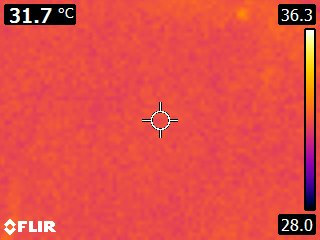
\includegraphics[scale = 0.5]{assets/figures/thermique_sans_chauffe.jpg}
        \caption{Image thermique du capteur - Corps de chauffe éteint}
    \end{subfigure}
    \hspace{0.2cm}
    \begin{subfigure}{0.3\textwidth}
        \centering
        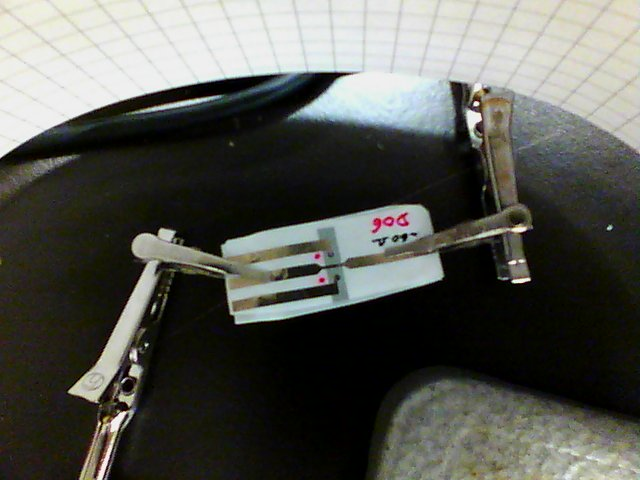
\includegraphics[scale = 0.23]{assets/figures/visuel_avec_chauffe.jpg}
        \caption{Image numérique}
    \end{subfigure}
    \hspace{0.5cm}
    \begin{subfigure}{0.3\textwidth}
        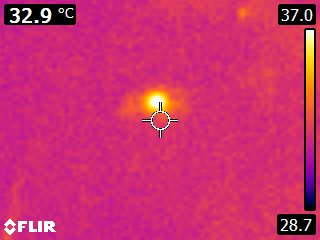
\includegraphics[scale = 0.5]{assets/figures/thermique_avec_chauffe.jpg}
        \caption{Image thermique du capteur - Corps de chauffe allumé}
    \end{subfigure}
    \caption{Résultats de la caméra thermique}
    \label{fig:cameraThermique}
\end{figure}

Il faut savoir que les pistes d'or réfléchissent énormément. Il est donc difficile d'obtenir un résultat parfait. Une première astuce a été de
dessiner au stylo un point noir sur les pistes à mesurer. Ainsi, les problèmes de réflexions seraient amoindris. Malheureusement cette astuce n'a
pas été suffisante. \\

Une autre mesure a alors été faite dans des conditions moins lumineuses (après le coucher du soleil). La figure \ref*{fig:cameraThermique},
montre que le corps de chauffe de l'échantillon D06 possède une température avoisinant les 37\textdegree C. \\

Un second type de mesure permettant de comprendre chaque partie du \gls{capteur} a été effectuée. Celle-ci concerne la résistance du corps de
chauffe et du circuit thermoélectrique.
\begin{table}[H]
    \begin{center}
        \begin{tabular}{|p{2cm}|p{2.5cm}|p{2.5cm}|p{2.5cm}|p{2.5cm}|}
            \hline
            Échantillon & \multicolumn{2}{|c|}{Corps de chauffe} & \multicolumn{2}{|c|}{Circuit du thermocouple}                                                                          \\
            \hline
                        & Résistance directe [$\Omega$]          & Résistance pointes ressorts [$\Omega$]        & Résistance directe [$\Omega$] & Résistance pointes ressorts [$\Omega$] \\
            \hline
            D06         & 74.29                                  & 75.3                                          & 151.5                         & 157                                    \\
            \hline
            D11         & 2.8                                    & 2.7                                           & 35 000 000                    & 20 000 000                             \\
            \hline
            D12         & 2.44                                   & 2.45                                          & 5600                          & 5580                                   \\
            \hline
            D13         & 6.07                                   & 6.14                                          & 585.5                         & 570.2                                  \\
            \hline
            D14         & 2.53                                   & 2.58                                          & 6.83                          & 6.91                                   \\
            \hline
            D17         & 9.2                                    & 9.4                                           & 13.6                          & 14                                     \\
            \hline
        \end{tabular}
        \caption{Résistances sur le capteur}
        \label{tab:resistancePointeRessort}
    \end{center}
\end{table}
Sur le tableau \ref*{tab:resistancePointeRessort}, une légère différence entre la résistance mesurée directement sur la piste d'or (résistance 
appelée Résistance directe) et la résistance à travers les pointes ressort est visible. Ceci peut être dû au fait que les pointes ressort ont 
également une petite résistance qui vient alors changer la résistance totale du corps de chauffe. Cependant, il faut également prendre en 
compte le fait que la résistance change suivant la position de la mesure. En effet, une mesure faite aux extrémités de la piste d'or sera différente 
d'une mesure effectuée sur le centre de la piste d'or. \\

L'échantillon D11 possède une résistance de thermocouple très instable et élevée. Pour cette raison, il a été décidé que les mesures ne seront 
pas effectuées, car ce capteur a peu de chance de donner des résultats concluants. 

Les tests de chauffe à la caméra ont été effectué sur d'autres échantillons tels que les échantillons D12, D13 et D14. Malheureusement ces derniers 
n'ont donné aucun résultat à la caméra thermique (aucun signe d'échauffement). Le corps de chauffe devra donc être amélioré en épaississant la 
couche d'or formé par la \gls{pvd} et/ou en modifiant la forme générale du corps de chauffe. 

\subsection{Hypothèses concernant l'échantillon pathologique}
Afin de détecter où se situe le problème, les différents paramètres du capteur \gls{capteur} ont été remis en question :
\begin{itemize}
    \item \textbf{Matériau thermoélectrique (ThEl)}\\
          La solution de Tellure de Bismuth est peut-être impure. Une nouvelle solution a été alors refaite.
          
    \item \textbf{Distance des pistes d'or du capteur au corps de chauffe}\\
          La distance entre le corps de chauffe et les piste d'or peut être importante, car trop proches, les unes des autres, la chaleur du corps
          de chauffe risque de se transmettre aux deux extrémités du capteur. De ce fait, la même température sera mesurable en tout point du
          capteur, n'engendrant donc aucune différence de température entre la partie droite et la partie gauche du \gls{capteur}, et donc aucune
          tension ne sera mesurable.\\
          
    \item \textbf{Épaisseur de la membrane} \\
          Plus la membrane est épaisse, plus la couche d'or de court-circuit sera éloignée. Cela permettrait à la source de chaleur d'être concentrée
          à un endroit spécifique. Ceci est important pour des raisons similaires au premier paramètre cité. Un transfert de chaleur faible (voir
          inexistant) entre les deux extrémités du \gls{capteur} est souhaitable (c'est la différence de température qui va engendrer une tension
          mesurable). \\
          
          Dans le stock de matière de membranes se trouvent les choix suivants :
          \begin{itemize}
              \item GTTP 6-10 $\mu$m d'épaisseur
              \item VCTP 6-10 $\mu$m d'épaisseur
              \item PI25005 25 $\mu$m d'épaisseur
          \end{itemize}
          L'objectif sera alors de faire des capteurs en PI25005 (Kepton) et de les comparer grâce au banc de test aux échantillons en GTTP ou VCTP.
          Ceci permettra d'affirmer ou désaffirmer l'hypothèse.\\
          
    \item \textbf{Diamètre du via}\\
          Lors de l'électrodéposition, un joint en caoutchouc percé au centre d'un diamètre de 0.3 mm, 0.5 mm ou 1 mm (appelé diamètre du via) permet de concentrer
          l'électrodéposition aux endroits souhaités. Cependant, si le diamètre du via est trop faible, l'électrodéposition peut avoir du mal à
          se produire (phénomènes de bulles, électrodéposition non-régulière, etc.)\\
          
    \item \textbf{Position de la piste de court-circuit}\\
          Afin de s'assurer que le corps de chauffe transmette un minimum de chaleur au deux extrémités du capteur, il serait possible de placer la couche
          d'or de court-circuit plus distante aux électrodépositions
\end{itemize}

\begin{comment}
\section{Résultats concluants}
Avec une nouvelle solution de Tellure de Bismuth et deux nouvelles électrodépositions sur une membrane de GTTP, de nouvelles mesures ont été
effectuées. Ces mesures nous ont montré que le capteur fonctionnait. En effet, une réponse a été mesurée.
\begin{table}[H]
    \begin{center}
        \begin{tabular}{|c|c|}
            \hline
            Condition du capteur                                   & Tension mesurée à travers l'amplificateur \\
            \hline
            Corps de chauffe désactivé et arrivée d'air désactivée & 5 mV                                      \\
            \hline
            Corps de chauffe activé et arrivée d'air désactivée    & 0 V                                       \\
            \hline
            Corps de chauffe activé et arrivée d'air activée       & 8 mV                                      \\
            \hline
        \end{tabular}
    \end{center}
\end{table}
Malgré le bruit non-négligeable mesuré à travers l'amplificateur, la tension change suivant les conditions du capteur. Afin de se concentrer
uniquement sur la réponse du capteur, l'amplificateur a été mis de côté pour les futures mesures.
\end{comment}

\section{Procédure de mesures "classiques"}
\begin{enumerate}
    \item Mesure avec un corps de chauffe pulsé\\
    \item Mesure avec un corps de chauffe pulsé et un flux d'air comprimé constant\\
    \item Mesure avec un flux d'air comprimé pulsé et un corps de chauffe constant\\
    \item Mesure sans corps de chauffe et une respiration humaine\\
    \item Mesure avec corps de chauffe constant et respiration humaine
\end{enumerate}
Ces mesures ont été effectuées sur quatre échantillons décrits au chapitre \ref{chap:capteur}. 

\section{Mesures du capteur sans amplificateur}
Plusieurs mesures ont été faites avec plusieurs types de paramètres. Toutes les mesures avec leurs paramètres ont été regroupées et sauvegardées
dans un document Excel qui se trouve en annexe.\\
Chacune des mesures sur cet Excel est liée à un autre fichier contenant toutes les valeurs concernant cette mesure.
\begin{figure}[H]
    \centering
    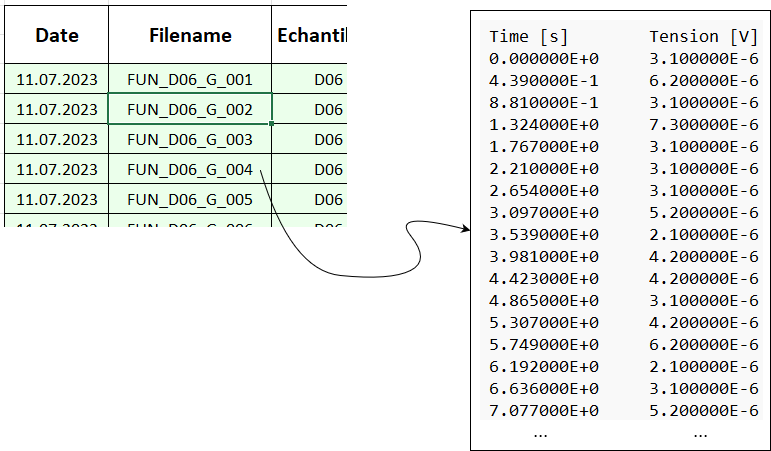
\includegraphics[scale = 0.4]{assets/figures/Data.png}
    \caption{Organisation des données}
    \label{fig:data_orga}
\end{figure}

Les mesures les plus significatives seront présentées dans ce rapport. \\

\subsection{Résultats avec un corps de chauffe pulsé}
Des premières mesures ont été effectuées sans flux d'air. En effet, il est déjà intéressant d'observer le comportement du capteur
lorsque seulement le corps de chauffe est activé. Ce dernier est alimenté avec 15 mA. Les résultats sont les suivants :
\begin{figure}[H]
    \hspace{-0.5cm}
    \begin{subfigure}[b]{0.45\textwidth}
        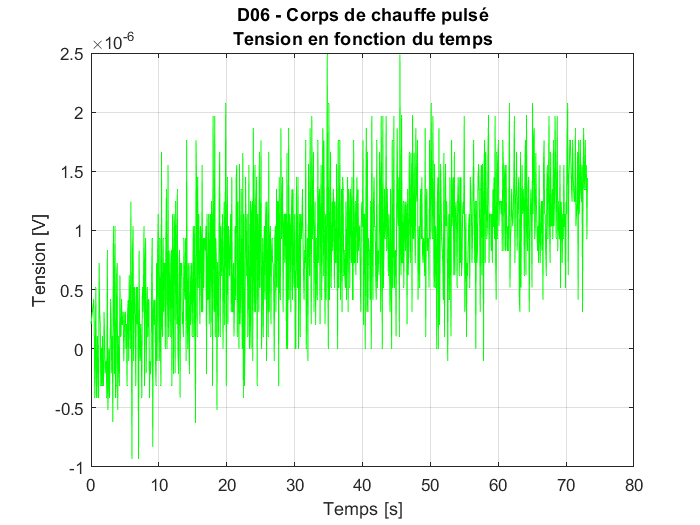
\includegraphics[scale = 0.45]{assets/figures/D06_corps_chauffe_pulse_green.png}
        \caption{Support Design 5 - Corps de chauffe pulsé}
        \label{fig:chauffe_pulse_g}
    \end{subfigure}
    \begin{subfigure}[b]{0.45\textwidth}
        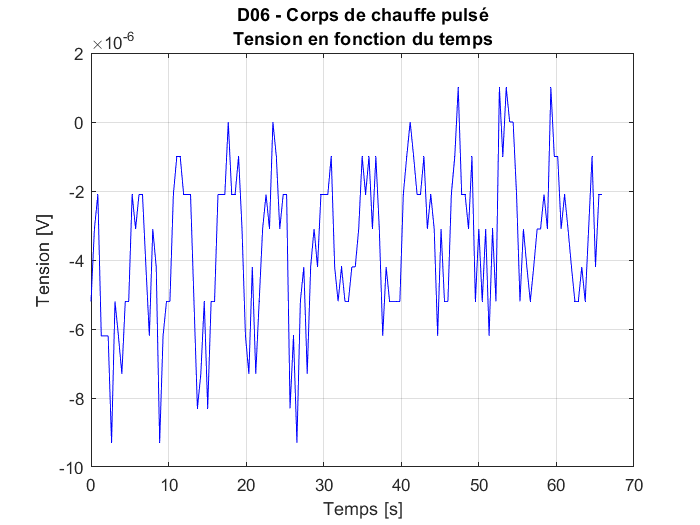
\includegraphics[scale = 0.45]{assets/figures/D06_corps_chauffe_pulse_blue.png}
        \caption{Support Design 1 - Corps de chauffe pulsé}
        \label{fig:chauffe_pulse_b}
    \end{subfigure}
\end{figure}

Sur la figure \ref{fig:chauffe_pulse_g}, aucun signal n'est distinguable. En effet, il semble n'y avoir que du bruit. Cependant, sur la figure
\ref{fig:chauffe_pulse_b}, la tension est bien moins stable. Pourtant, aucun flux n'est encore ajouté. \\

La raison de ce phénomène peut se trouver dans le fait que chaque électrodéposition est faite à la main, une après l'autre. Ceci signifie que
les deux électrodépositions diffèrent certainement l'une de l'autre. \\
De plus, le corps de chauffe est assez proche des deux électrodépositions. De ce fait, il est probable que lorsqu'il est en marche, le corps de
chauffe transfert de la chaleur aux deux extrémités du capteur. Ces deux extrémités sont alors chauffées, mais comme elles possèdent des nanofils
quelque peu différents d'un côté ou de l'autre, un gradient de température se forme et une certaine tension circule. \\
C'est une hypothèse du phénomène que l'on peut observer sur la figure \ref{fig:chauffe_pulse_b}.\\

Le support Design 5 semble, lui, éviter ce transfert de chaleur. Cela peut être dû au fait qu'étant donné que la membrane est plaquée contre
la pièce du support, la chaleur transférée par le corps de chauffe est "perdue" dans la matière du support (ici : PLA).\\

Pour ces raisons, le support Design 1 a été privilégié étant donné qu'il semblait plus sensible que le support Design 5.\\

\subsection{Mesures avec corps de chauffe constant et flux d'air comprimé pulsé}
\begin{figure}[H]
    \centering
    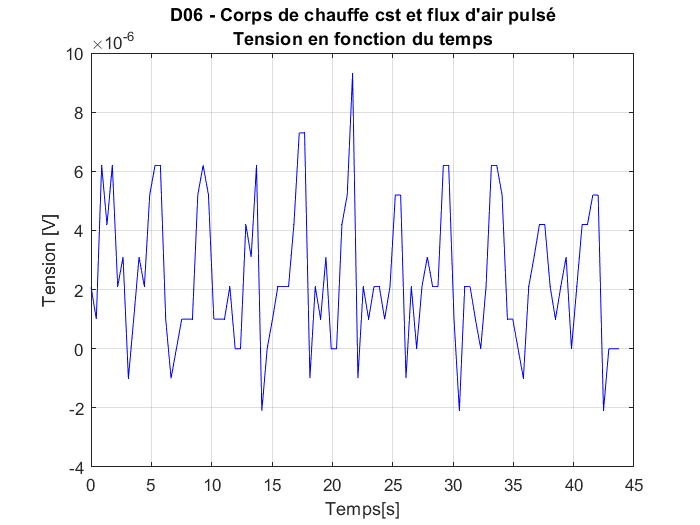
\includegraphics[scale = 0.5]{assets/figures/D06_air_comprime_pulse.png}
    \caption{Échantillon D06 - Flux d'air comprimé pulsé (corps de chauffe constant)}
    \label{fig:D06_airPulse}
\end{figure}
La figure \ref{fig:D06_airPulse}, montre la réponse du capteur lorsqu'un flux d'air comprimé vient souffler sur le capteur pendant 3 s, puis 
stoppe le flux d'air pendant également 3 s. 

\begin{figure}[H]
    \centering
    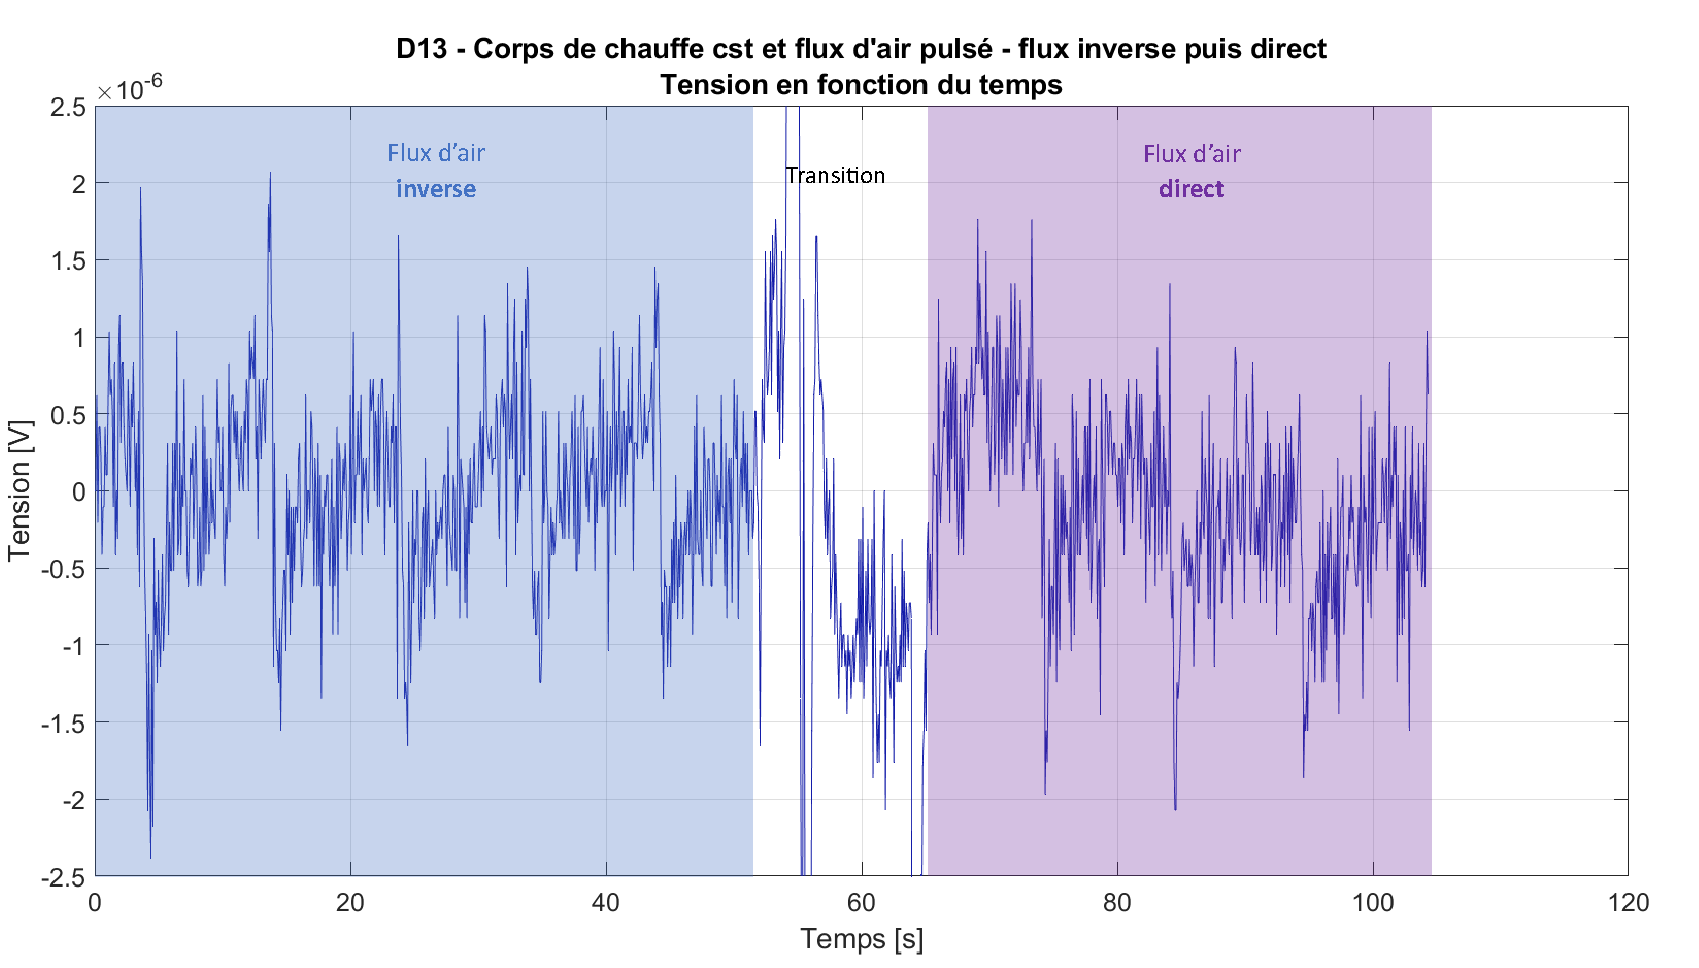
\includegraphics[scale = 0.6]{assets/figures/D13_air_comprime_pulse_blue.pdf}
    \caption{Échantillon D13 - Flux d'air comprimé pulsé en sens inverse puis direct}
    \label{fig:D13_air_comp_pulse}
\end{figure}

Sur la figure \ref{fig:D13_air_comp_pulse}, la fréquence du souffle d'air comprimé est la même que pour la figure précédente 
(\ref{fig:D06_airPulse}). Cependant, après environ 50 s, le tube d'arrivée d'air est débranché pour venir se rebrancher dans l'autre sens 
du capteur. 

\begin{figure}[H]
    \centering
    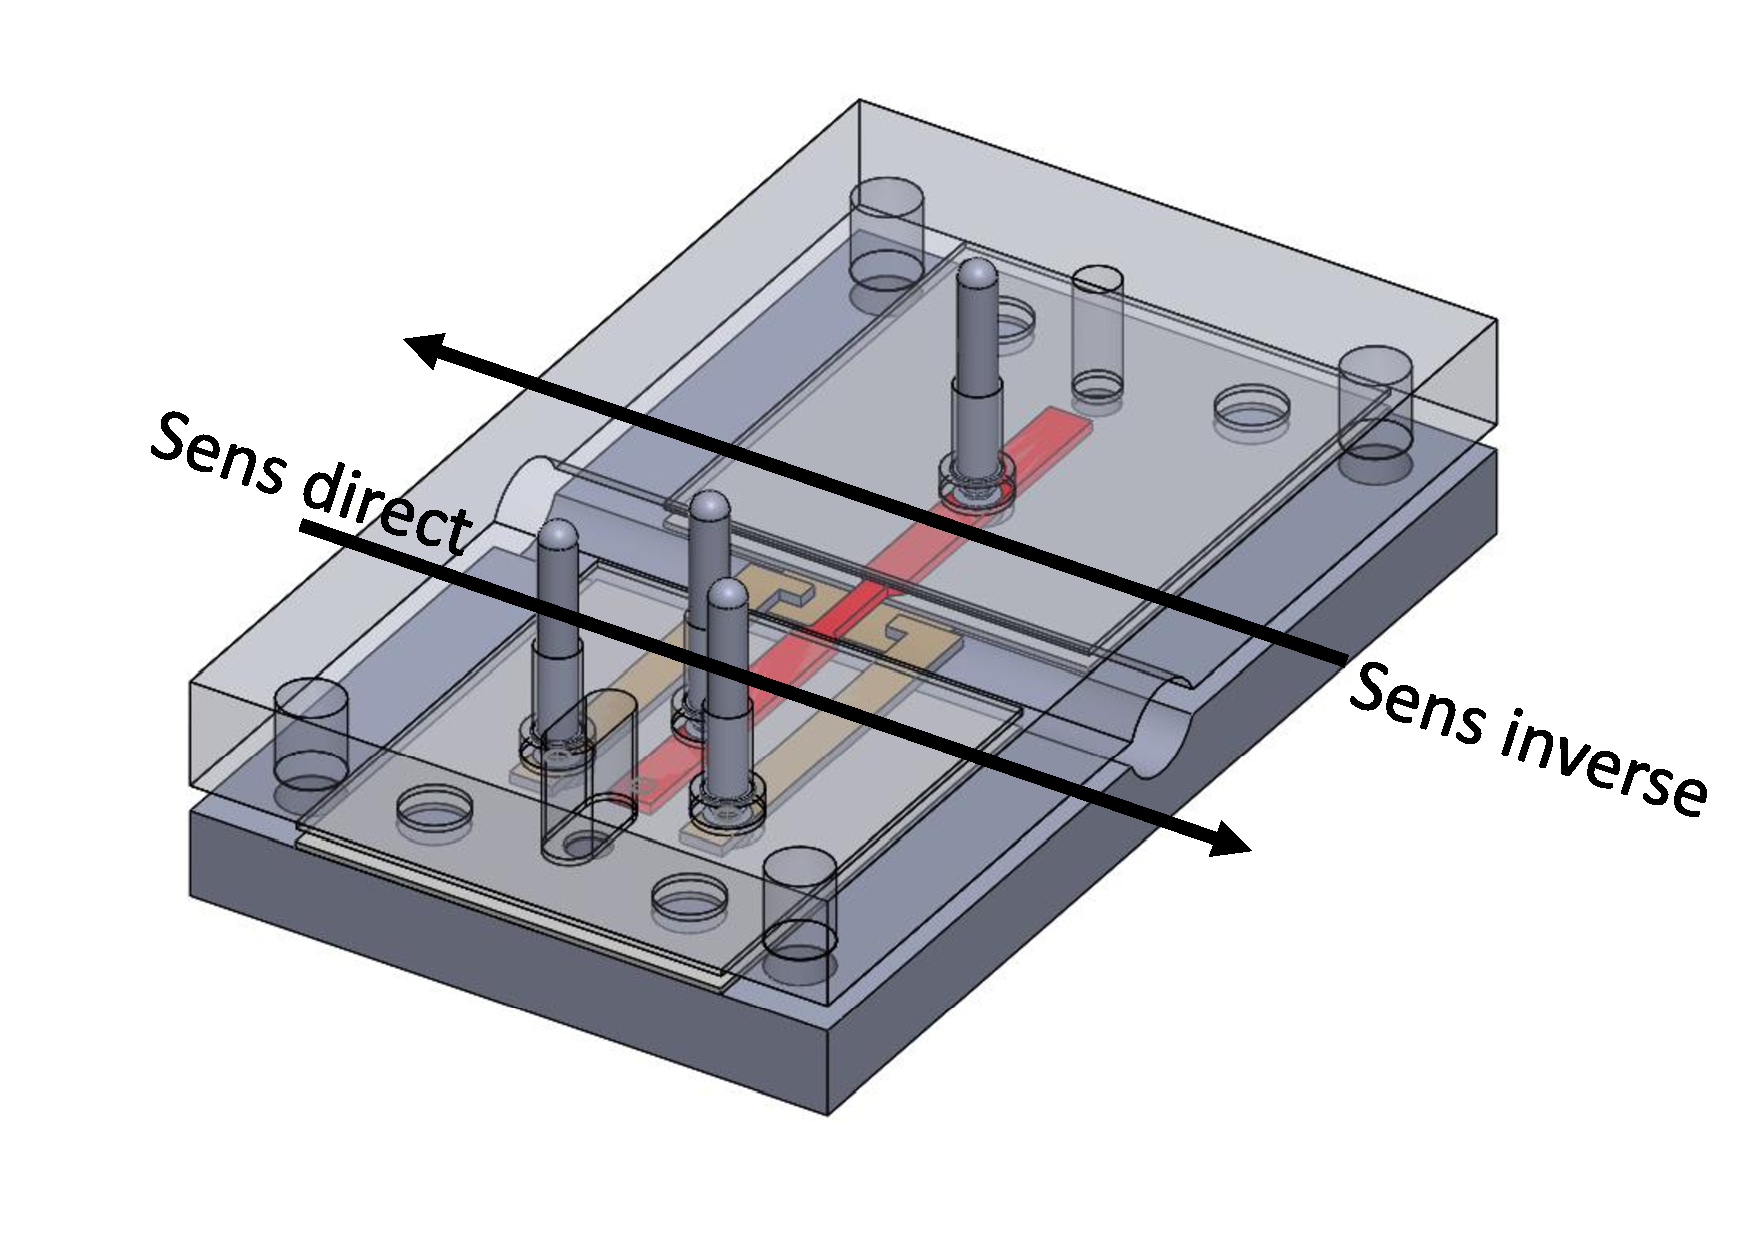
\includegraphics[scale = 0.3]{assets/figures/Inverse_direct.pdf}
    \caption{Sens direct ou inverse du flux d'air}
    \label{fig:direct_inverse}
\end{figure}

Cette manipulation permet d'observer si un comportement différent est à noter. Dans notre cas, l'allure du graphe semble peu changer d'un sens 
ou de l'autre. Les électrodépositions sont alors assez différentes du côté droit que du côté gauche pour générer un signal lorsque seulement un 
corps de chauffe pulsé et utilisé, mais pas complètement dissemblables, jusqu'à obtenir des résultats qui diffèrent d'un sens ou de l'autre. 

\subsection{Respiration humaine}
Au lieu d'amener le flux d'air par une source d'air comprimé, l'arrivée d'air sera effectué par une respiration humaine. Ceci nous a donné les résultats suivants :

\begin{figure}[H]
    \centering
    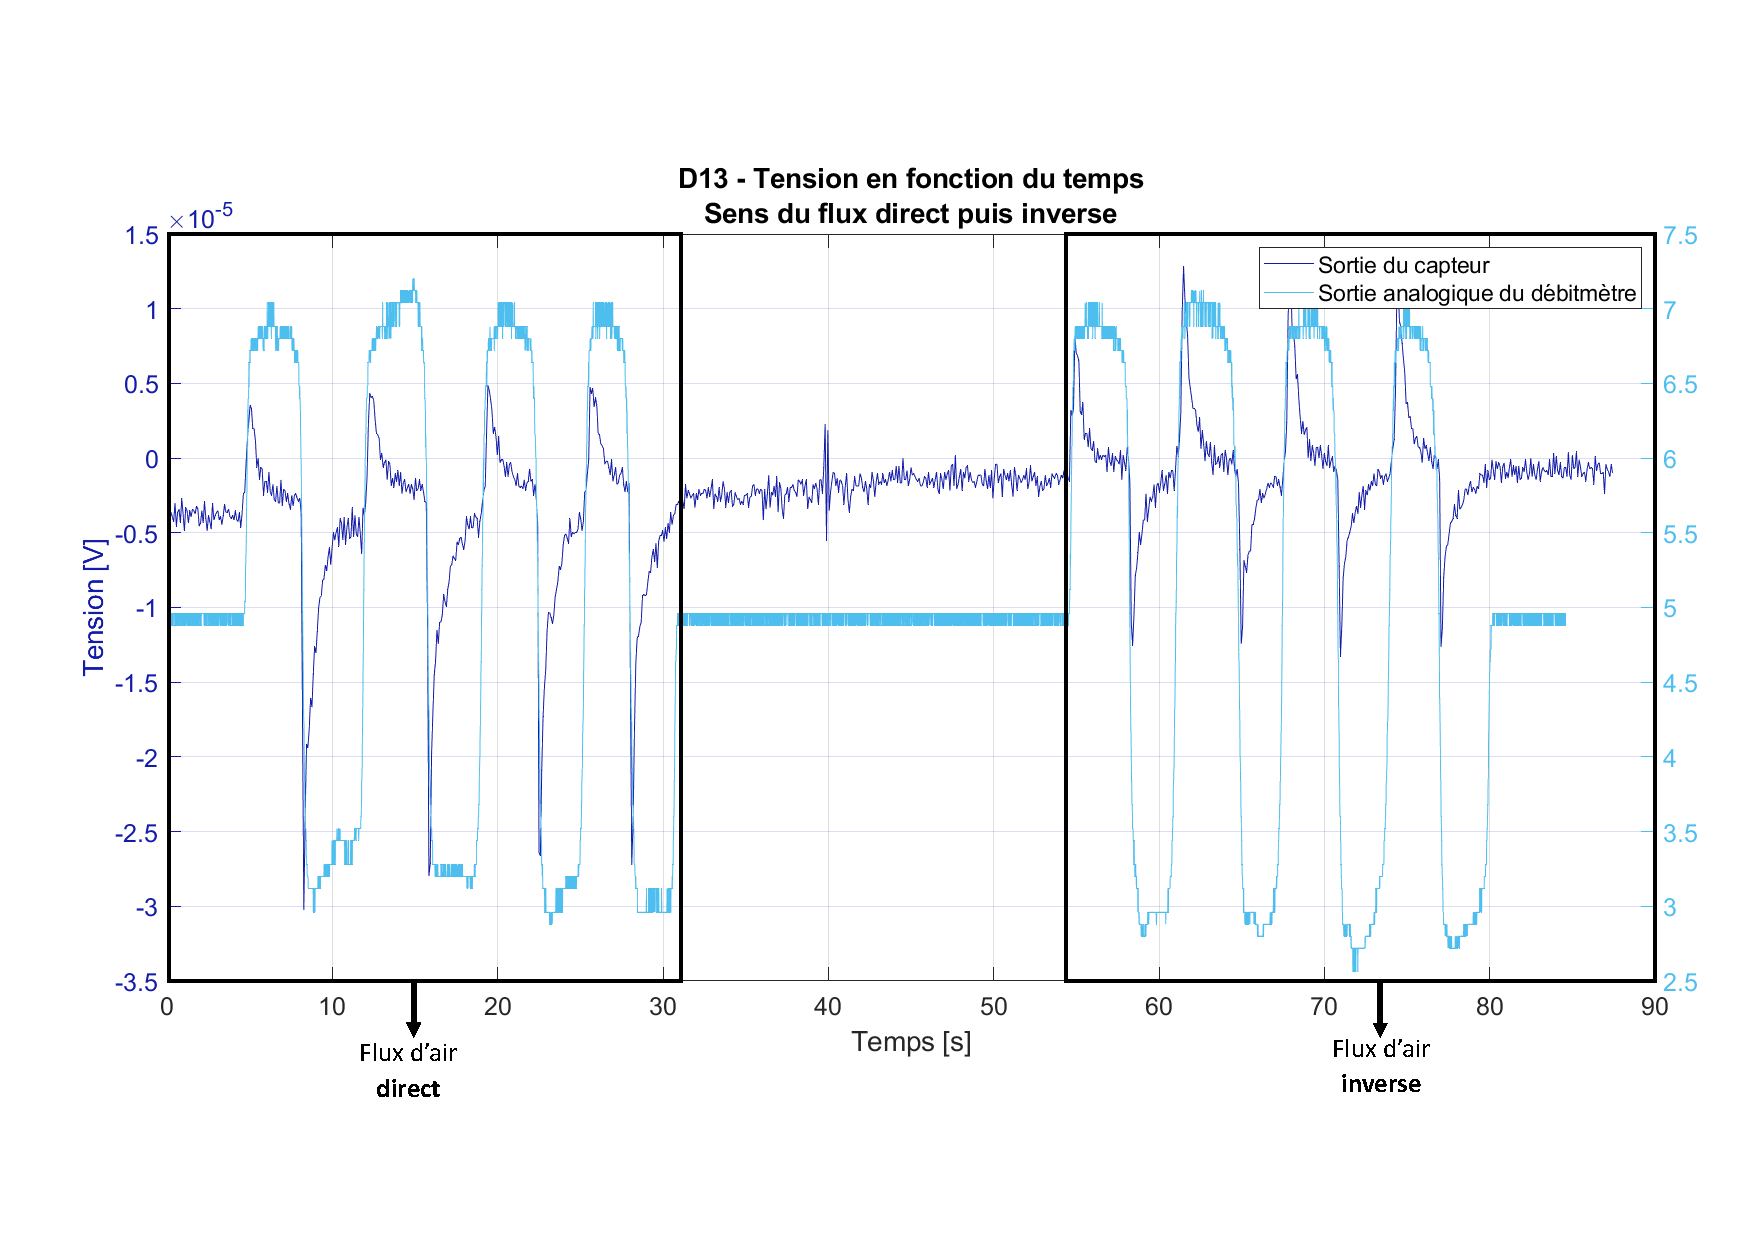
\includegraphics[scale = 0.6]{assets/figures/D13_human_breath_direct_invert_blue.pdf}
    \caption{D13 - Réponse du capteur à la respiration humaine en sens direct et inverse}
    \label{fig:D13_human_breath_direct_invert}
\end{figure}

La partie gauche du graphe de la figure \ref{fig:D13_human_breath_direct_invert}, correspond à la réponse du capteur et du débitmètre lorsque la 
respiration se fait en sens direct. La partie droite, quant à elle, montre ces deux mêmes réponses, mais lorsque la respiration se fait en sens 
inverse (cf. figure \ref{fig:direct_inverse}). 

Les mesures de la respiration humaine avec et sans corps de chauffe ont montré très peu de différences. Ainsi, le corps de chauffe a été laissé 
de côté pour le moment. 

\subsection{Mesure concernant la condensation}
Les résultats avec la respiration humaine sont bien plus nettes que ceux avec l'air comprimé. Ce phénomène peut être dû au fait que le capteur 
est sensible à l'humidité (en plus de la chaleur). De plus, étant donné que le comportement est différent lors de l'inspiration ou l'expiration, 
il était intéressant d'émettre quelques hypothèses :
\begin{itemize}
    \item L'expiration humaine est constituée d'air humide chaud qui vient donc réchauffer et humidifier le capteur
    \item L'humidité vient se déposer sur la membrane
    \item Lors de l'inspiration, il y aura un phénomène d'évaporation qui viendra changer à nouveau la température du capteur
\end{itemize}

Afin d'étudier ces hypothèses, une expérience a été effectuée en expirant seulement pendant quelques secondes (ici 5 s), puis en laissant le 
capteur reposer un certain temps. Cette manipulation permettrait d'observer si l'humidité de l'expiration s'évapore (si tel est le cas, le 
capteur devrait montrer quelque chose après l'expiration, mais avant le retour au zéro). 
\begin{comment}
\begin{figure}[H]
    \centering
    \includegraphics[scale = 0.5]{name}
    \caption{title}
    \label{fig:}
\end{figure}
\end{comment}

\section{Dépendances}
\section{Discussion}
